\chapter{Grundlagen}
In diesem Kapitel werden die zentralen Begriffe und Methoden ausführlich vorgestellt. So wird das notwendige Grundlagenwissen vermittelt, auf dem die weitere Ausarbeitung aufbaut.

\section{Vier-Gewinnt}
Das Spiel Vier-Gewinnt wird auf einem Spielfeldraster mit sechs Zeilen und sieben Spalten gespielt. Zum Spielbeginn erhält jeder Spieler 21 Spielchips, entweder Rote oder Gelbe. Ziel des Spiels ist es, möglichst schnell vier Chips der eigenen Farbe in eine Reihe zu bringen – waagrecht, senkrecht oder diagonal. Die Spieler werfen abwechselnd ihre Chips in das Spielfeld, bis entweder ein Spieler das Ziel erreicht oder alle 42 Felder belegt sind \autocite{Hasbro.2020}.

\section{Alpha-Beta-Pruning-Algorithmus}
Alpha-Beta-Pruning ist ein Verfahren, das bei Spielen wie Schach, Dame oder Vier Gewinnt eingesetzt wird, um den optimalen nächsten Zug zu bestimmen. Ziel des Algorithmus ist es, die Suche im Spielbaum effizienter zu machen. Im Unterschied zum Minimax-Algorithmus werden beim Alpha-Beta-Pruning gezielt Teilbäume weggelassen, die für das Endergebnis keine Rolle spielen.
Während der Tiefensuche durch den Spielbaum arbeitet der Algorithmus mit zwei Schrankenwerten, dem Alpha ($\alpha$) und dem Beta ($\beta$). Zu Beginn wird Alpha auf $-\infty$ und Beta auf $+\infty$ gesetzt.
An jedem MAX-Knoten wird das Maximum aus dem bisherigen Alpha und den Werten der Nachfolgeknoten ausgewählt. Das bedeutet, Alpha wird immer dann erhöht, wenn ein nachfolgender Knoten einen höheren Wert liefert als das aktuelle Alpha.
Am MIN-Knoten hingegen wird Beta jeweils auf das Minimum aus dem bisherigen Beta und den Werten der Nachfolgeknoten gesetzt.
Sobald an einem Knoten die Bedingung $\alpha \geq \beta$ erfüllt ist, wird der restliche Teilbaum nicht weiter betrachtet. In diesem Fall hat der MIN bereits eine bessere Alternative gefunden, sodass MAX diesen Zweig des Baums nicht mehr wählen würde \autocite{adorf2009alphabeta}.


\begin{figure}[H]
	\centering
	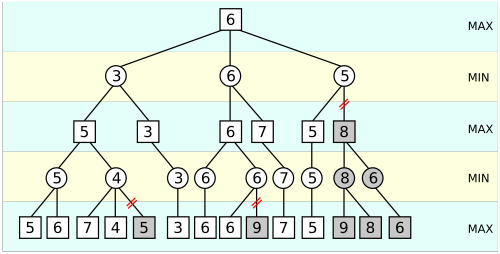
\includegraphics[width=1\linewidth]{images/alpha_beta}
	\caption[Alpha-Beta Spielbaum Quelle: \autocite{wikimediaABpruning}]{Alpha-Beta Spielbaum}
	\label{fig:alphabeta}
\end{figure}



\section{Mikropython}
MicroPython ist eine speziell für Mikrocontroller angepasste Version der Programmiersprache Python. Im Gegensatz zur Desktop-Variante lässt sich MicroPython-Code direkt auf Hardware mit begrenzten Ressourcen ausführen\autocite{energy_responsiveness2023}\autocite{Plauska2023}.\
Im Unterschied zu Standard-Python 3 bringt MicroPython allerdings nur einen Teil der gewohnten Python-Standardbibliotheken mit.\\ Wodurch es weniger Speicherplatz benötigt.
Zudem besitzt MicroPython einen eigenen Interpreter, der direkt auf einem Mikrokontroller ausgeführt werden kann.
Dadurch eignet sich MicroPython besonders gut für die Programmierung des LEGO Spike Hubs\autocite{bell2024micropython}.



\section{LEGO Spike Komponenten}
In diesem Kapitel werden die zentralen LEGO Spike-Komponenten beschrieben, die beim Bau des Roboters verwendet wurden. 

\subsection{Hub}
Der LEGO Spike Hub ist das Herzstück des LEGO Spike Prime Sets. Er dient als programmierbare Steuereinheit mit sechs LPF2 input/output ports, an die alle LEGO-Sensoren und -Motoren angeschlossen werden können. Im Inneren arbeitet ein eigener Prozessor (100 MHz ARM Cortex-M4), unterstützt von 320 KB RAM und 1 MB Flash-Speicher. Die Programmierung des LEGO Spike Hubs erfolgt in der Sprache MicroPython. LEGO stellt dafür eine eigene Entwicklungsumgebung (IDE) bereit, mit dieser der Hub einfach programmiert werden kann. Hierfür kann der Hub über USB oder via Bluetooth mit dem Computer verbunden werden. Die Steuereinheit wird über einen  wiederaufladbarer Lithium-Ionen-Akku mit Strom und Spannung versorgt \autocite{lego2020techniclargehub}.

Weitere technische Merkmale des LEGO Spike Hubs sind:
\begin{itemize}
	\item Individuell anpassbaren Lichtmatrix (5x5)
	\item Lautsprecher
	\item Taster mit integrierter Statusleuchte 
	\item Tasten für die Navigation und Steuerung durch Menüs am Hub 
	\item Lautsprecher
	\item sechsachsiger Gyrosensor 
\end{itemize} 

\begin{figure}[H]
	\centering
	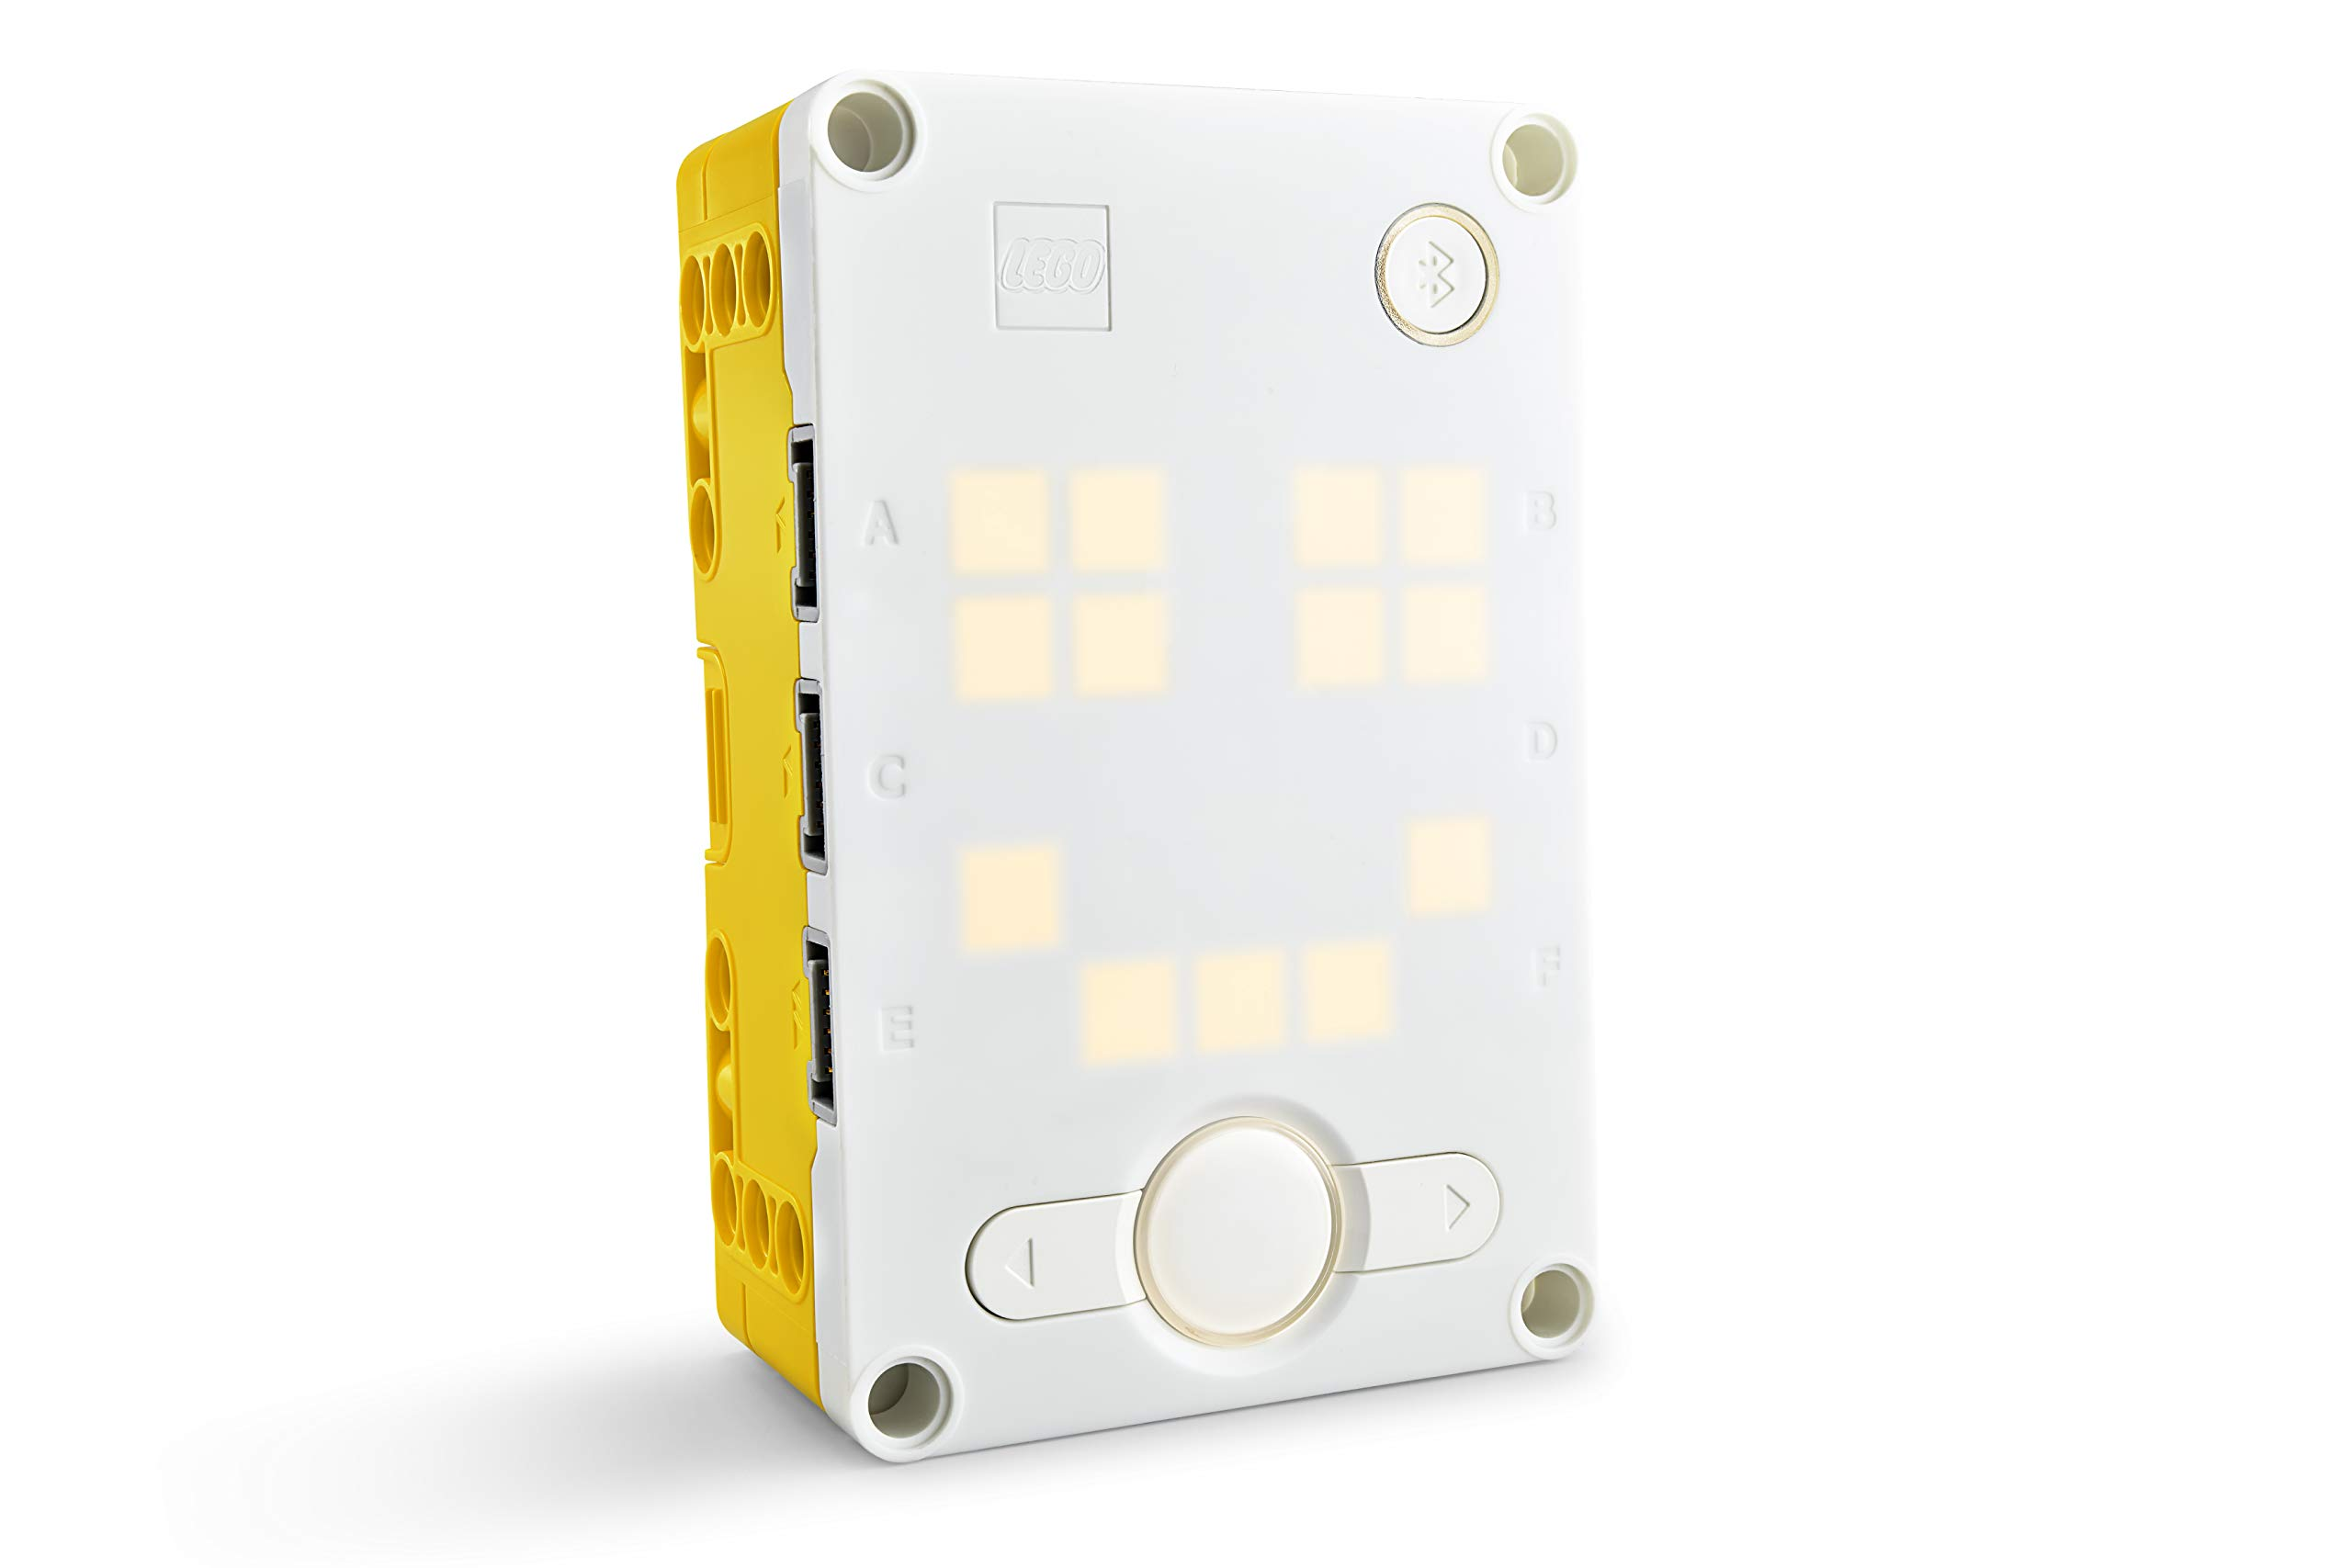
\includegraphics[width=0.55\linewidth]{images/Hub}
	\caption[LEGO Spike Hub Quelle:\autocite{legoeducation2020spikesensors}]{LEGO Spike Hub}
	\label{fig:hub}
\end{figure}

\subsection{LEGO Spike Kraft- oder Touchsensor}
Dieser Sensor erkennt, ob er gedrückt wurde, und misst dabei gleichzeitig die auf ihn ausgeübte Kraft. Mit einer Abtastrate von 100 Hz erfasst er Kräfte im Bereich von 2,5 bis 10 Newton und arbeitet dabei mit einer Genauigkeit von $\pm 0,65$ Newton. Der gemessene Wert wird als Prozentwert ausgegeben, wobei 100\% einem Tastendruck von 10 Newton entsprechen. Typischerweise wird der Sensor zum Erkennen von Hindernissen oder als Start- bzw. Stopptaste eines Roboters eingesetzt. Der Kraft- oder Tuchsensor wird direkt am LEGO Spike Hub angeschlossen \autocite{legoeducation2020spikesensors}.

\begin{figure}[H]
	\centering
	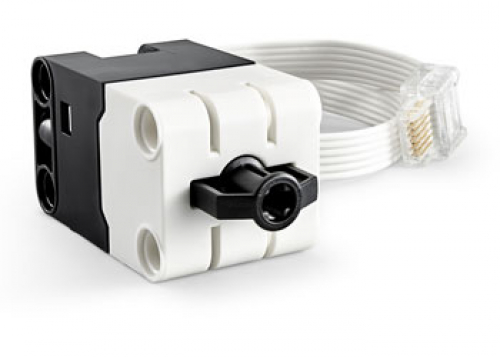
\includegraphics[width=0.4\linewidth]{images/Kraftsensor}
	\caption[LEGO Spike Kraft- oder Touchsensor Quelle:\autocite{legoeducation2020spikesensors}]{LEGO Spike Kraft- oder Touchsensor}
	\label{fig:kraftsensor}
\end{figure}

\subsection{LEGO Spike Farbsensor}
Dieser elektronische Farbsensor wurde speziell für LEGO Spike entwickelt. Seine Abtastrate beträgt 1 kHz und er kann direkt am Hub angeschlossen werden. Der Sensor kann bis zu acht verschiedene Farben erkennen, darunter Schwarz, Blau, Rot, Weiß, Braun, Gelb, Pink und Grün. Außerdem misst er sowohl die Intensität des reflektierten Lichts als auch die des Umgebungslichts \autocite{lego2020colorsensor}\autocite{legoeducation2020spikesensors}.

Für die Farberkennung erfasst der Sensor die Farbwerte sowohl im RGB- (Rot, Grün, Blau) als auch im HSV-Farbraum (hue = Farbton, saturation = Sättigung, value = Helligkeit). Die Messergebnisse werden als Ganzzahlen ausgegeben \autocite{lego2020colorsensor}.

Zur Reflexionsmessung sendet der Sensor weißes Licht auf eine Oberfläche und misst das zurückgeworfene Licht. Diese Funktion wird häufig für Linienführung eingesetzt \autocite{betzold2025colorsensor}\autocite{lego2020colorsensor}.

\begin{figure}[H]
	\centering
	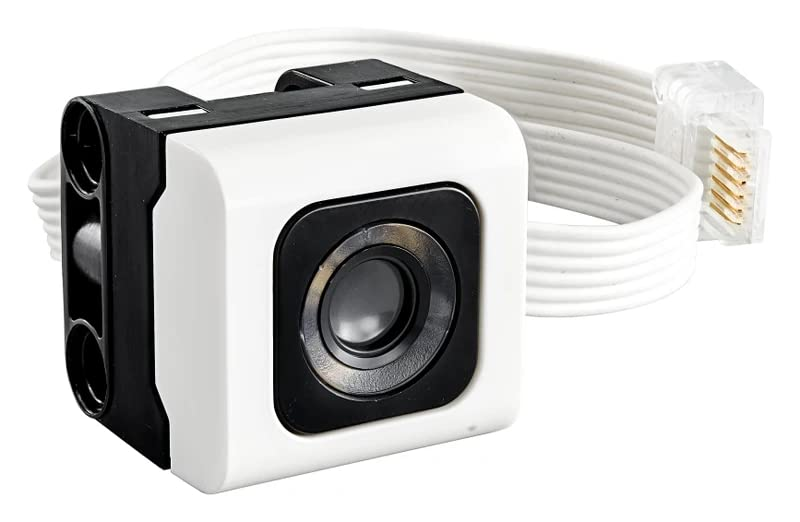
\includegraphics[width=0.4\linewidth]{images/Farbsensor}
	\caption[LEGO Technic Farbsensor Quelle:\autocite{legoeducation2020spikesensors}]{LEGO Technic Farbsensor}
	\label{fig:farbsensor}
\end{figure}

\subsection{LEGO Spike Winkelmotor}
Der LEGO Spike Winkelmotor ist nicht nur ein einfacher Elektromotor, aufgrund eines integrierten Drehsensors kann er nicht nur die Drehrichtung, sondern auch die relative und absolute Position (in Grad) sowie die Drehgeschwindigkeit erfassen. Eine vollständige Umdrehung wird dabei in 360 einzelne Zählimpulse unterteilt, wobei die Genauigkeit des Motors bei $\pm3$ Grad liegt. Muss der Motor ein Drehmoment von mehr als 5 Ncm aufbringen, blockiert er. Mit einer Abtastrate von 100 Hz erfasst der Motor die Position sowohl beim automatischen als auch im manuellen Betrieb. Der LEGO Spike Winkelmotor eignet sich somit nicht nur für Bewegungsaufgaben, sondern auch zur Positionsbestimmung \autocite{legoeducation2020spikesensors}.

\begin{figure}[H]
	\centering
	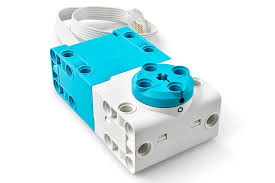
\includegraphics[width=0.4\linewidth]{images/Motor}
	\caption[LEGO Spike Winkelmotor Quelle:\autocite{legoeducation2020spikesensors}]{LEGO Spike Winkelmotor}
	\label{fig:motor}
\end{figure}

